\documentclass[11pt]{article}

\usepackage[margin=1in]{geometry}
\usepackage{amsmath, amssymb}
\usepackage{graphicx}
\usepackage{enumitem}
\usepackage{fancyhdr}
\usepackage{hyperref}
\usepackage{minted}

\pagestyle{fancy}
\fancyhf{}
\lhead{ENPM701 --- Homework 5}
\rhead{Marcus Hurt}
\cfoot{\thepage}

\title{Homework 5}
\author{Marcus Hurt \\ \href{mailto:mhurt@umd.edu}{mhurt@umd.edu}}
\date{ENPM701: Autonomous Robotics}

\begin{document}

\begin{titlepage}
    \centering
    \vspace*{2in}
    {\LARGE\bfseries Homework 5\par}
    \vspace{0.5in}
    {\Large ENPM701: Autonomous Robotics\par}
    \vspace{1in}
    {\large Marcus Hurt\par}
    \href{mailto:mhurt@umd.edu}{mhurt@umd.edu}
    \vfill
    {\large University of Maryland\par}
    {\large \today\par}
\end{titlepage}

\section*{Question \#1 (5 points)}

The video details the potential benefits of using a LIDAR or cameras for autonomous vehicles. LIDAR offers a point cloud output that can penetrate some mediums that cameras cannot, such as fog, rain, and darkness. LIDAR is also not fooled by visual artifacts like a picture of the road, which can cause cameras to misinterpret the environment as shown in the pinnacle experiment of the video where a camera system ran into a foam wall while the LIDAR system stopped before impact.

LIDAR systems passed all six tests in the video, while the camera system failed three of them. Three of the tests (rain, fog, bright light) could be argued that humans would not pass. The second test (a child running into the road) is simply a case of reation time, so a human may fail here as well while both camera and LIDAR systems passed. The tests exemplify benefits for each system, with a camera conceivably improving human reaction time and a LIDAR system improving performance in adverse conditions.

The video brings the question of expectations of vehicle safety systems to the discussion. Are safety systems expected to perform equivalently to a human driver, improve a human driver, or perform outright better than a human driver? A camera system could be argued to be equivalent to a human in most aspects, with visual analysis of the environment, the camera system would be expected to react faster than an average human driver, but it is vulnerable to visual artifacts and adverse conditions. This means it would be reasonable to always expect human oversight of a camera system.

A LIDAR system could be argued to perform better than a human driver in most aspects, with the ability to penetrate adverse conditions and not be fooled by visual artifacts. This means it would be reasonable to expect a LIDAR system to perform without human oversight, as it would be expected to outperform a human driver and a camera system in most scenarios. While not addressed in the video, the use of sensor fusion to combine a camera and LIDAR system would be a topic of interest, as it could potentially combine the benefits of both systems while mitigating their weaknesses.

\section*{Question \#2 (20 points)}

The in class exercise can be seen in figure \ref{fig:in_class_exercise}.

\begin{figure}[h]
    \centering
    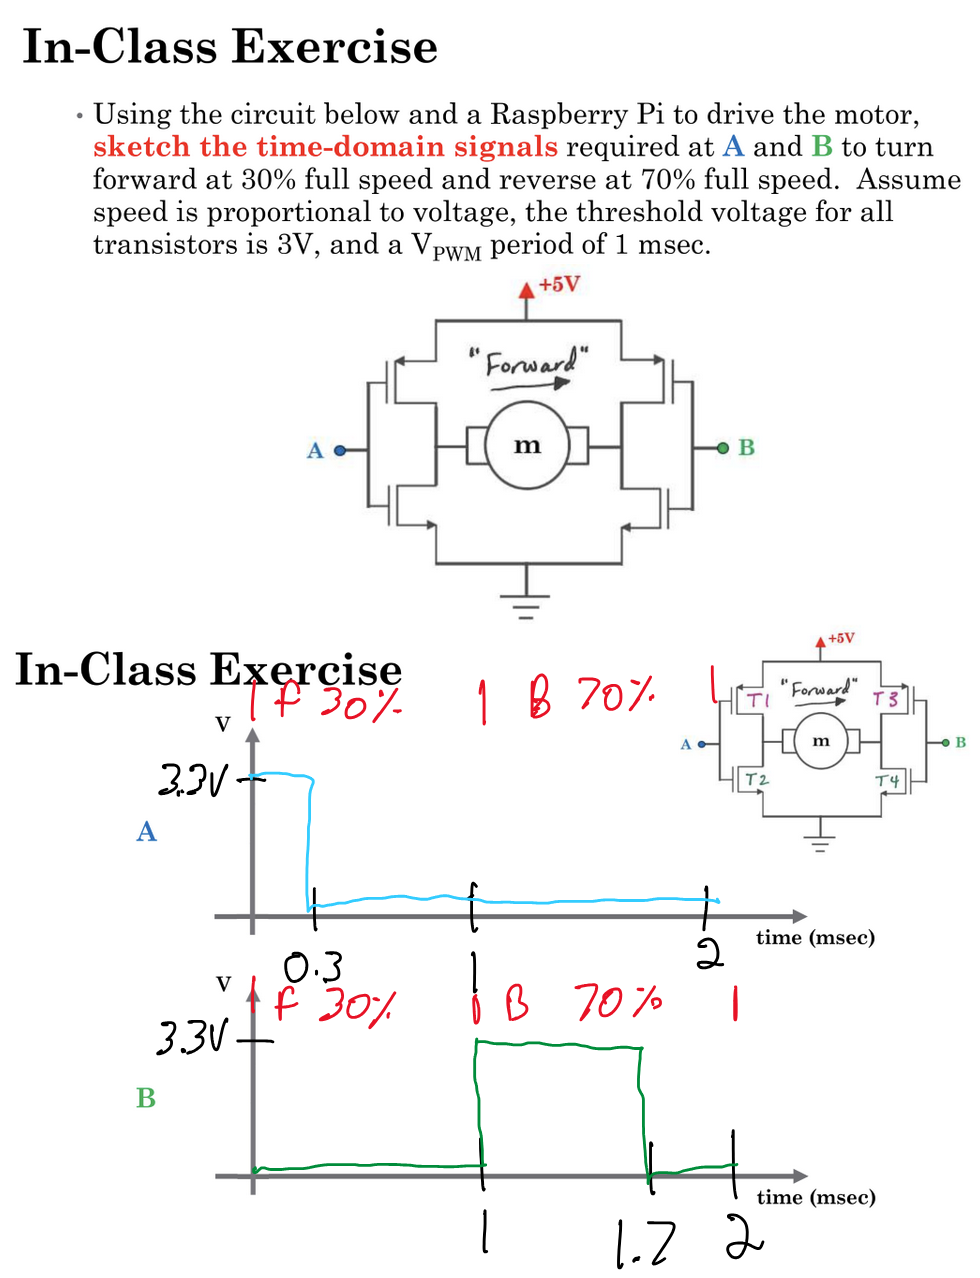
\includegraphics[width=0.8\textwidth]{InClass.png}
    \caption{In Class Exercise}
    \label{fig:in_class_exercise}
\end{figure}

See the video at the following link for a demonstration of the robot driving.

\url{https://youtube.com/shorts/oYMHYw86KHM}

\section*{Question \#3 (5 points)}

The Burro system lists vision and GPS as the navigation sensors. It advertises both online route creation and management as well as destination based navigation. It also advertises obstacle stopping, avoidance, and path planning with its vision system.

Complex tasks like autonomous routes and docking advertise a combination of GPS and vision. This makes sense as GPS can provide a general location and route, while vision can provide more detailed information about the environment for obstacle avoidance and precise navigation. The use of both sensors allows for a more robust and reliable navigation system, as it can leverage the strengths of each sensor to compensate for their weaknesses.

A fascinating note that may only partially be related to the navigation and localization is that the Burro advertises data collection of up to 1 TB per hour. This is an enormous amount of data, raising the question of what is it used for. The RICOH360 camera can store 900 RAW+ images with a storage capacity of 51 GB. In the burrow this would be almost 18,000 images per hour or 5 fps video. Without further speculation, this detail was of interest and worth noting.

\end{document}